% Options for packages loaded elsewhere
\PassOptionsToPackage{unicode}{hyperref}
\PassOptionsToPackage{hyphens}{url}
%
\documentclass[
]{article}
\usepackage{amsmath,amssymb}
\usepackage{iftex}
\ifPDFTeX
  \usepackage[T1]{fontenc}
  \usepackage[utf8]{inputenc}
  \usepackage{textcomp} % provide euro and other symbols
\else % if luatex or xetex
  \usepackage{unicode-math} % this also loads fontspec
  \defaultfontfeatures{Scale=MatchLowercase}
  \defaultfontfeatures[\rmfamily]{Ligatures=TeX,Scale=1}
\fi
\usepackage{lmodern}
\ifPDFTeX\else
  % xetex/luatex font selection
\fi
% Use upquote if available, for straight quotes in verbatim environments
\IfFileExists{upquote.sty}{\usepackage{upquote}}{}
\IfFileExists{microtype.sty}{% use microtype if available
  \usepackage[]{microtype}
  \UseMicrotypeSet[protrusion]{basicmath} % disable protrusion for tt fonts
}{}
\makeatletter
\@ifundefined{KOMAClassName}{% if non-KOMA class
  \IfFileExists{parskip.sty}{%
    \usepackage{parskip}
  }{% else
    \setlength{\parindent}{0pt}
    \setlength{\parskip}{6pt plus 2pt minus 1pt}}
}{% if KOMA class
  \KOMAoptions{parskip=half}}
\makeatother
\usepackage{xcolor}
\usepackage[margin=1in]{geometry}
\usepackage{longtable,booktabs,array}
\usepackage{calc} % for calculating minipage widths
% Correct order of tables after \paragraph or \subparagraph
\usepackage{etoolbox}
\makeatletter
\patchcmd\longtable{\par}{\if@noskipsec\mbox{}\fi\par}{}{}
\makeatother
% Allow footnotes in longtable head/foot
\IfFileExists{footnotehyper.sty}{\usepackage{footnotehyper}}{\usepackage{footnote}}
\makesavenoteenv{longtable}
\usepackage{graphicx}
\makeatletter
\def\maxwidth{\ifdim\Gin@nat@width>\linewidth\linewidth\else\Gin@nat@width\fi}
\def\maxheight{\ifdim\Gin@nat@height>\textheight\textheight\else\Gin@nat@height\fi}
\makeatother
% Scale images if necessary, so that they will not overflow the page
% margins by default, and it is still possible to overwrite the defaults
% using explicit options in \includegraphics[width, height, ...]{}
\setkeys{Gin}{width=\maxwidth,height=\maxheight,keepaspectratio}
% Set default figure placement to htbp
\makeatletter
\def\fps@figure{htbp}
\makeatother
\setlength{\emergencystretch}{3em} % prevent overfull lines
\providecommand{\tightlist}{%
  \setlength{\itemsep}{0pt}\setlength{\parskip}{0pt}}
\setcounter{secnumdepth}{5}
\newlength{\cslhangindent}
\setlength{\cslhangindent}{1.5em}
\newlength{\csllabelwidth}
\setlength{\csllabelwidth}{3em}
\newlength{\cslentryspacingunit} % times entry-spacing
\setlength{\cslentryspacingunit}{\parskip}
\newenvironment{CSLReferences}[2] % #1 hanging-ident, #2 entry spacing
 {% don't indent paragraphs
  \setlength{\parindent}{0pt}
  % turn on hanging indent if param 1 is 1
  \ifodd #1
  \let\oldpar\par
  \def\par{\hangindent=\cslhangindent\oldpar}
  \fi
  % set entry spacing
  \setlength{\parskip}{#2\cslentryspacingunit}
 }%
 {}
\usepackage{calc}
\newcommand{\CSLBlock}[1]{#1\hfill\break}
\newcommand{\CSLLeftMargin}[1]{\parbox[t]{\csllabelwidth}{#1}}
\newcommand{\CSLRightInline}[1]{\parbox[t]{\linewidth - \csllabelwidth}{#1}\break}
\newcommand{\CSLIndent}[1]{\hspace{\cslhangindent}#1}
\usepackage{longtable}
\usepackage{booktabs}
\usepackage{graphicx}
\usepackage{float}
\usepackage{setspace}\onehalfspacing
\usepackage{booktabs}
\usepackage{longtable}
\usepackage{array}
\usepackage{multirow}
\usepackage{wrapfig}
\usepackage{float}
\usepackage{colortbl}
\usepackage{pdflscape}
\usepackage{tabu}
\usepackage{threeparttable}
\usepackage{threeparttablex}
\usepackage[normalem]{ulem}
\usepackage{makecell}
\usepackage{xcolor}
\ifLuaTeX
  \usepackage{selnolig}  % disable illegal ligatures
\fi
\IfFileExists{bookmark.sty}{\usepackage{bookmark}}{\usepackage{hyperref}}
\IfFileExists{xurl.sty}{\usepackage{xurl}}{} % add URL line breaks if available
\urlstyle{same}
\hypersetup{
  pdftitle={In it for the long run},
  pdfauthor={Rasmus H. Klokker},
  hidelinks,
  pdfcreator={LaTeX via pandoc}}

\title{In it for the long run}
\author{Rasmus H. Klokker}
\date{2024-08-16}

\begin{document}
\maketitle

\hypertarget{introduction}{%
\section{Introduction}\label{introduction}}

Teachers are the cornerstone of the educational system, and their career trajectories significantly impact the quality of education that students receive. Understanding these career paths can provide critical insights into the factors that influence teacher retention, professional development, and overall job satisfaction. Such knowledge can help policymakers and stakeholders who aim to improve educational outcomes and ensure a stable and effective teaching workforce.

Research on teacher career choices is intrinsically linked to issues of educational inequality. Teachers' decisions regarding where to work, whether to stay in the profession and how to advance their careers can exacerbate or alleviate disparities in educational opportunities(Glassow, Yang Hansen, and Gustafsson 2023). For instance, schools in low-income or rural areas often face higher turnover rates, leading to a lack of experienced and qualified teachers in these communities(Ingersoll and Tran 2023). This turnover can result in a cycle of educational disadvantage, where students in underprivileged areas receive lower-quality education than their peers in more affluent regions.

Moreover, teacher career paths are influenced by various factors such as working conditions, support systems, and professional development opportunities, which are often unevenly distributed across different schools and districts. Schools serving disadvantaged populations frequently lack the resources to provide the necessary support for teacher growth and retention, further perpetuating educational inequality. By examining these career trajectories, researchers can identify key interventions and policies that can support teachers more effectively, particularly in underserved areas.

While scholarly literature on teacher career choices has emerged, particularly within the literature on teacher sorting, knowledge on teacher career paths that span long time horizons is still minimal. As such, knowledge of teacher career paths does, in many cases, concern partial teacher careers rather than the entire careers of teachers, spanning entry to the labor market all the way to retirement.

In this paper, I will investigate patterns of teacher career paths using sequence analysis. Subsequently, I will use cluster analysis to form types of teacher career paths and investigate how teacher characteristics, such as teacher credentials, are associated with different types of teacher career paths.

Crucially, using high-quality Danish register data, I am able to follow cohorts of teacher graduates from the year of graduation onwards. Given that the earliest cohort graduated in 1980, I am able to investigate the career paths of teachers across several decades, enabling me to map out the full career paths of the earliest teacher cohorts.

\hypertarget{contribution}{%
\section{Contribution}\label{contribution}}

Thus, this paper will primarily contribute by expanding our knowledge on the late stages of teacher career paths. This includes the transitions from mid- to late-stage careers as well as how patterns of late-stage teacher careers compare to the early- and mid-stage teacher careers. Crucially, this will also contribute knowledge on the timing of teachers who opt out of teaching. If there exists a non-trivial share of teachers who opt out of teaching in the later stages of their career, earlier studies on teacher careers, and particularly teacher attrition, may underestimate the share of teachers who opt out of teaching. If, however, teachers who opt out of teaching in the earlier stages of their careers choose to enter teaching again later in their careers, previous studies could have overestimated the share of teachers who opt out of teaching indefinitely.

\hypertarget{research-questions}{%
\subsection{Research questions}\label{research-questions}}

In this paper, I will follow two overarching research questions.

\begin{enumerate}
\def\labelenumi{\arabic{enumi})}
\item
  How can individual teacher career choices be segmented to form distinct types of teacher career paths?
\item
  How are teacher characteristics associated with distinct types of teacher career paths?
\end{enumerate}

\hypertarget{findings}{%
\subsection{Findings}\label{findings}}

In this paper, I find that more than 50\% of teacher graduates choose to work outside public primary schools. Further, I find that teacher career paths can be divided into four general types of career paths:

\begin{enumerate}
\def\labelenumi{\arabic{enumi})}
\item
  A type of career path in which teachers almost exclusively work outside public primary schools.
\item
  A type of career path in which teachers primarily work in schools that serve less affluent students
\item
  A type of career path in which teachers primarily work in schools that serve the most affluent students
\item
  A type of career path in which teachers primarily work in schools that serve middle-class students
\end{enumerate}

Lastly, I find that teacher characteristics, measured at the time of graduation, are very poor predictors of which career path teachers choose to follow.

\hypertarget{state-of-the-art}{%
\subsection{State of the art}\label{state-of-the-art}}

This section will outline the current scholarly literature on teacher careers.

\hypertarget{what-do-we-know-about-how-teachers-change-jobs-throughout-their-career}{%
\subsection{What do we know about how teachers change jobs throughout their career?}\label{what-do-we-know-about-how-teachers-change-jobs-throughout-their-career}}

Few studies provide broad overviews of teacher career paths. In Gubler, Biemann, and Herzog (2017), we find the most broad overview. The authors find six different types of career paths. The majority of teachers start as primary school teachers before they transition to childcare and part-time work as public school teachers. The second most frequent career path type involves teachers with stable employment in primary school teaching across the entire period. While the study of Gubler, Biemann, and Herzog (2017) is closely related to this paper regarding the method and overall research goal, there are some key differences. Firstly, while the authors construct overall patterns of teacher careers using sequence analysis, the authors do not focus on transitions between schools serving different types of students, e.g., low- and high-SES students. Secondly, while the study can track teachers across a relatively long period of time(15 years), the sample size is limited to 999 teachers.

The remaining literature on teacher career paths focuses on more specific elements of teacher career choices or is more loosely related to research questions on teacher career paths.

For instance, Falch (2022), Goldhaber et al. (2022), and Boyd et al. (2002) all focus on the early careers of teachers. For Falch (2022) and Boyd et al. (2002), the focus is specifically on teacher attrition. Falch (2022) finds that attrition from teaching positions increases steadily as teachers gain experience and that teachers mainly pursue occupations outside teaching. Further, attrition was higher among teachers with higher degrees of academic ability, which is also among the results of Boyd et al. (2002). Goldhaber et al. (2022) found similar results regarding attrition but also found that a substantial proportion of newly graduated teachers enter employment outside public primary schools before transitioning to teaching positions.

There is a large scholarly literature that does not directly address teacher career paths. However, many of the results in this literature are relevant to the present paper, especially in regard to how school and teacher characteristics impact teachers' decisions to stay at or leave the school at which they are currently employed.

\hypertarget{what-do-we-know-about-how-teachers-change-jobs-between-schools-that-serve-different-kinds-of-students}{%
\subsection{What do we know about how teachers change jobs between schools that serve different kinds of students?}\label{what-do-we-know-about-how-teachers-change-jobs-between-schools-that-serve-different-kinds-of-students}}

There is considerable literature on how school characteristics, e.g., the composition of the student body, the school's physical environment, the work environment, the quality of school leadership, etc., impact teacher attrition and retention. Three comprehensive literature reviews,Guarino, Santibanez, and Daley (2006), Borman and Dowling (2008), and Nguyen et al. (2020), summarize this literature. However, Nguyen et al. (2020) is the most recent review and encompasses the studies included in the previous reviews. In Nguyen et al. (2020), comparisons of different types of schools, e.g., private vs.~public schools, middle school vs.~elementary school, etc., are consistently among the factors that increase the propensity for teachers to leave their current school the most. However, higher degrees of student disciplinary problems is the third highest effect size among the factors that increase attrition, with higher degrees of student discipline problems increasing the probability of leaving ones current school by about 16\%. Interestingly, there are more school characteristics that consistently lower teacher attrition. An improved work environment reduced the odds of leaving the current school by nearly 50\%, although the estimate is associated with a very high degree of uncertainty. While the effect sizes for providing induction/mentoring to newly hired teachers, opportunities for professional development, and administrative support are smaller, the effects are estimated with considerably less uncertainty than the effect of an improved work environment.
Interestingly, student body characteristics do not seem to impact teacher attrition to any discernable degree. Only the estimated effect of student poverty is of noticeable size, but due to the width of the confidence interval we cannot reject that student poverty might actually decrease teacher attrition.

\begin{figure}[H]
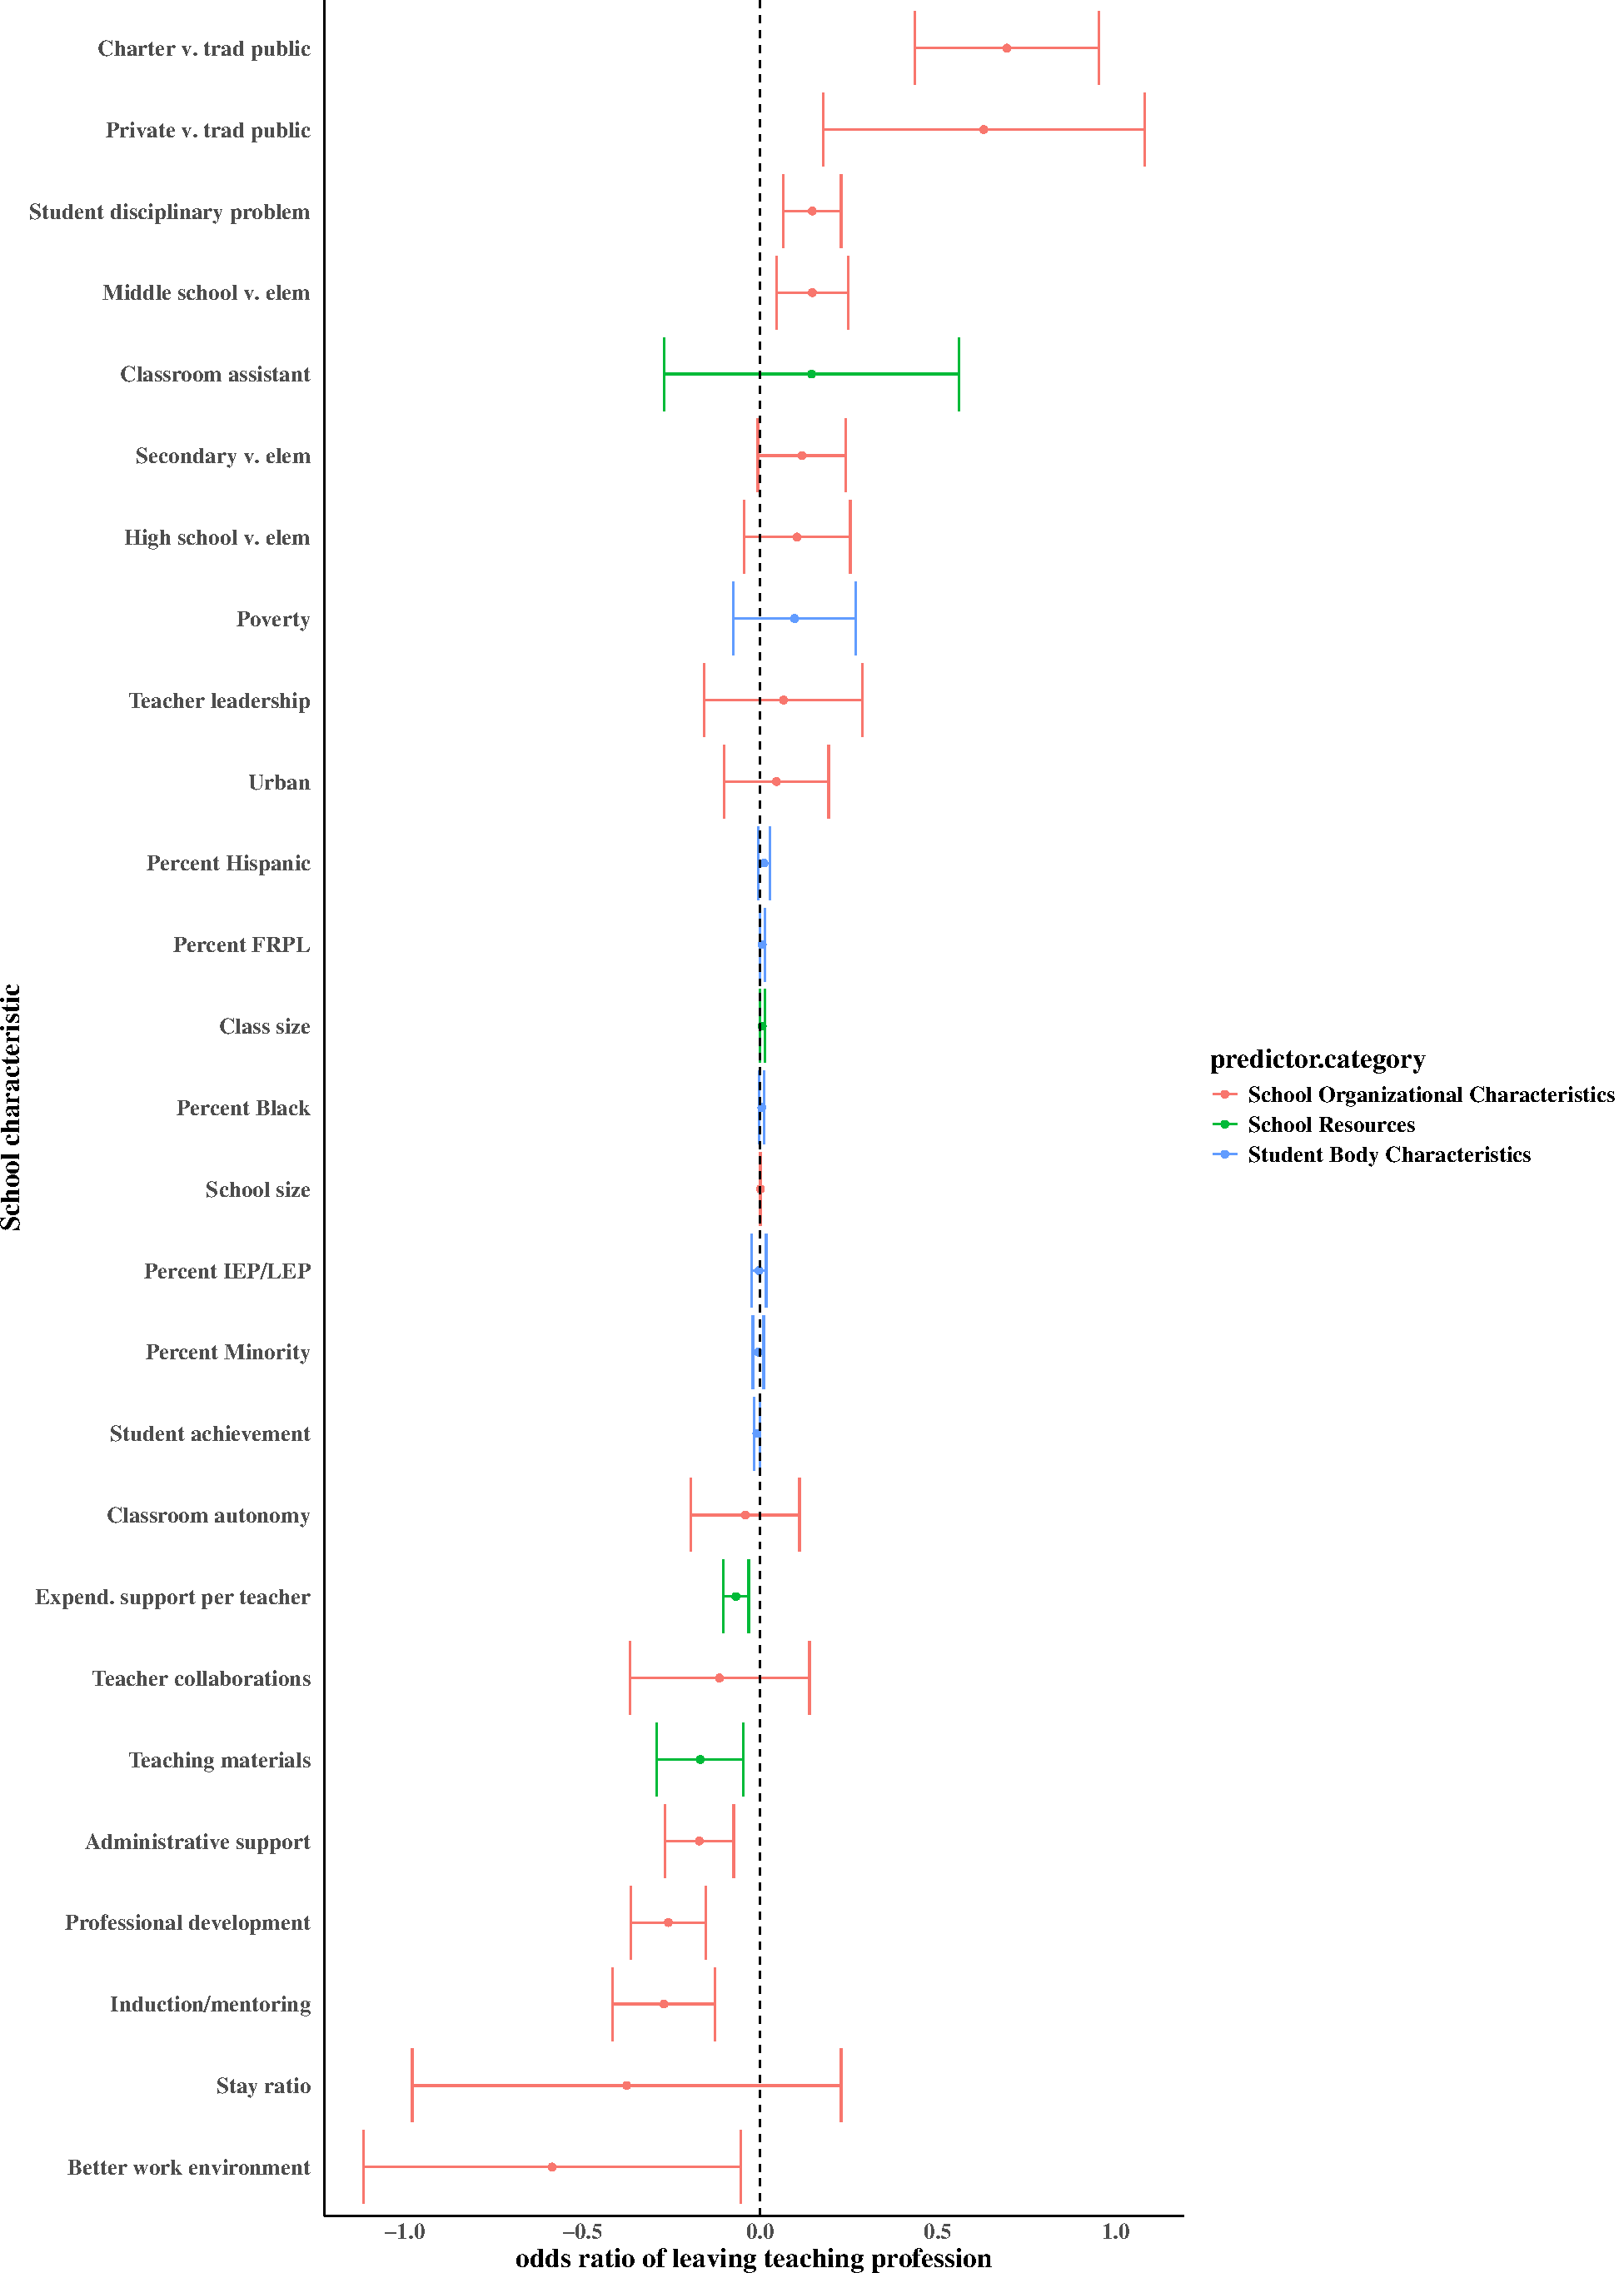
\includegraphics[width=1\linewidth,]{In-it-for-the-long-run_kollekolle_files/figure-latex/compare-effs-1} \caption{Associations between leaving the teaching profession and school characteristics - reproduced from Nguyen, 2020}\label{fig:compare-effs}
\end{figure}

\hypertarget{what-do-we-know-about-how-teacher-characteristics-impact-career-choices}{%
\subsection{What do we know about how teacher characteristics impact career choices?}\label{what-do-we-know-about-how-teacher-characteristics-impact-career-choices}}

Regarding teacher characteristics, the estimated effect of having more than three years of experience suggests that having more than three years of experience increases the odds of attrition by more than 48\%. Having a professional specialization also seems to increase the odds of teacher attrition, with teachers specializing in fields other than STEM or special education being the most at risk of attrition. Interestingly, having better test scores, e.g., SAT scores, only has a negligible effect on attrition of teachers. On the other end of the spectrum, having more children and having a teacher certification reduces the odds of attrition by about 50\%. Having a full-time teaching position, being in the Hispanic minority group, and being older than 28 years of age also reduces the odds of attrition considerably, all reducing the odds of attrition by more than 30\%. The effect sizes for the remaining factors are either too small to warrant any attention here or are not statistically significant. Thus, we cannot reject the fact that these effect sizes could be either positive or negative.

\begin{figure}[H]
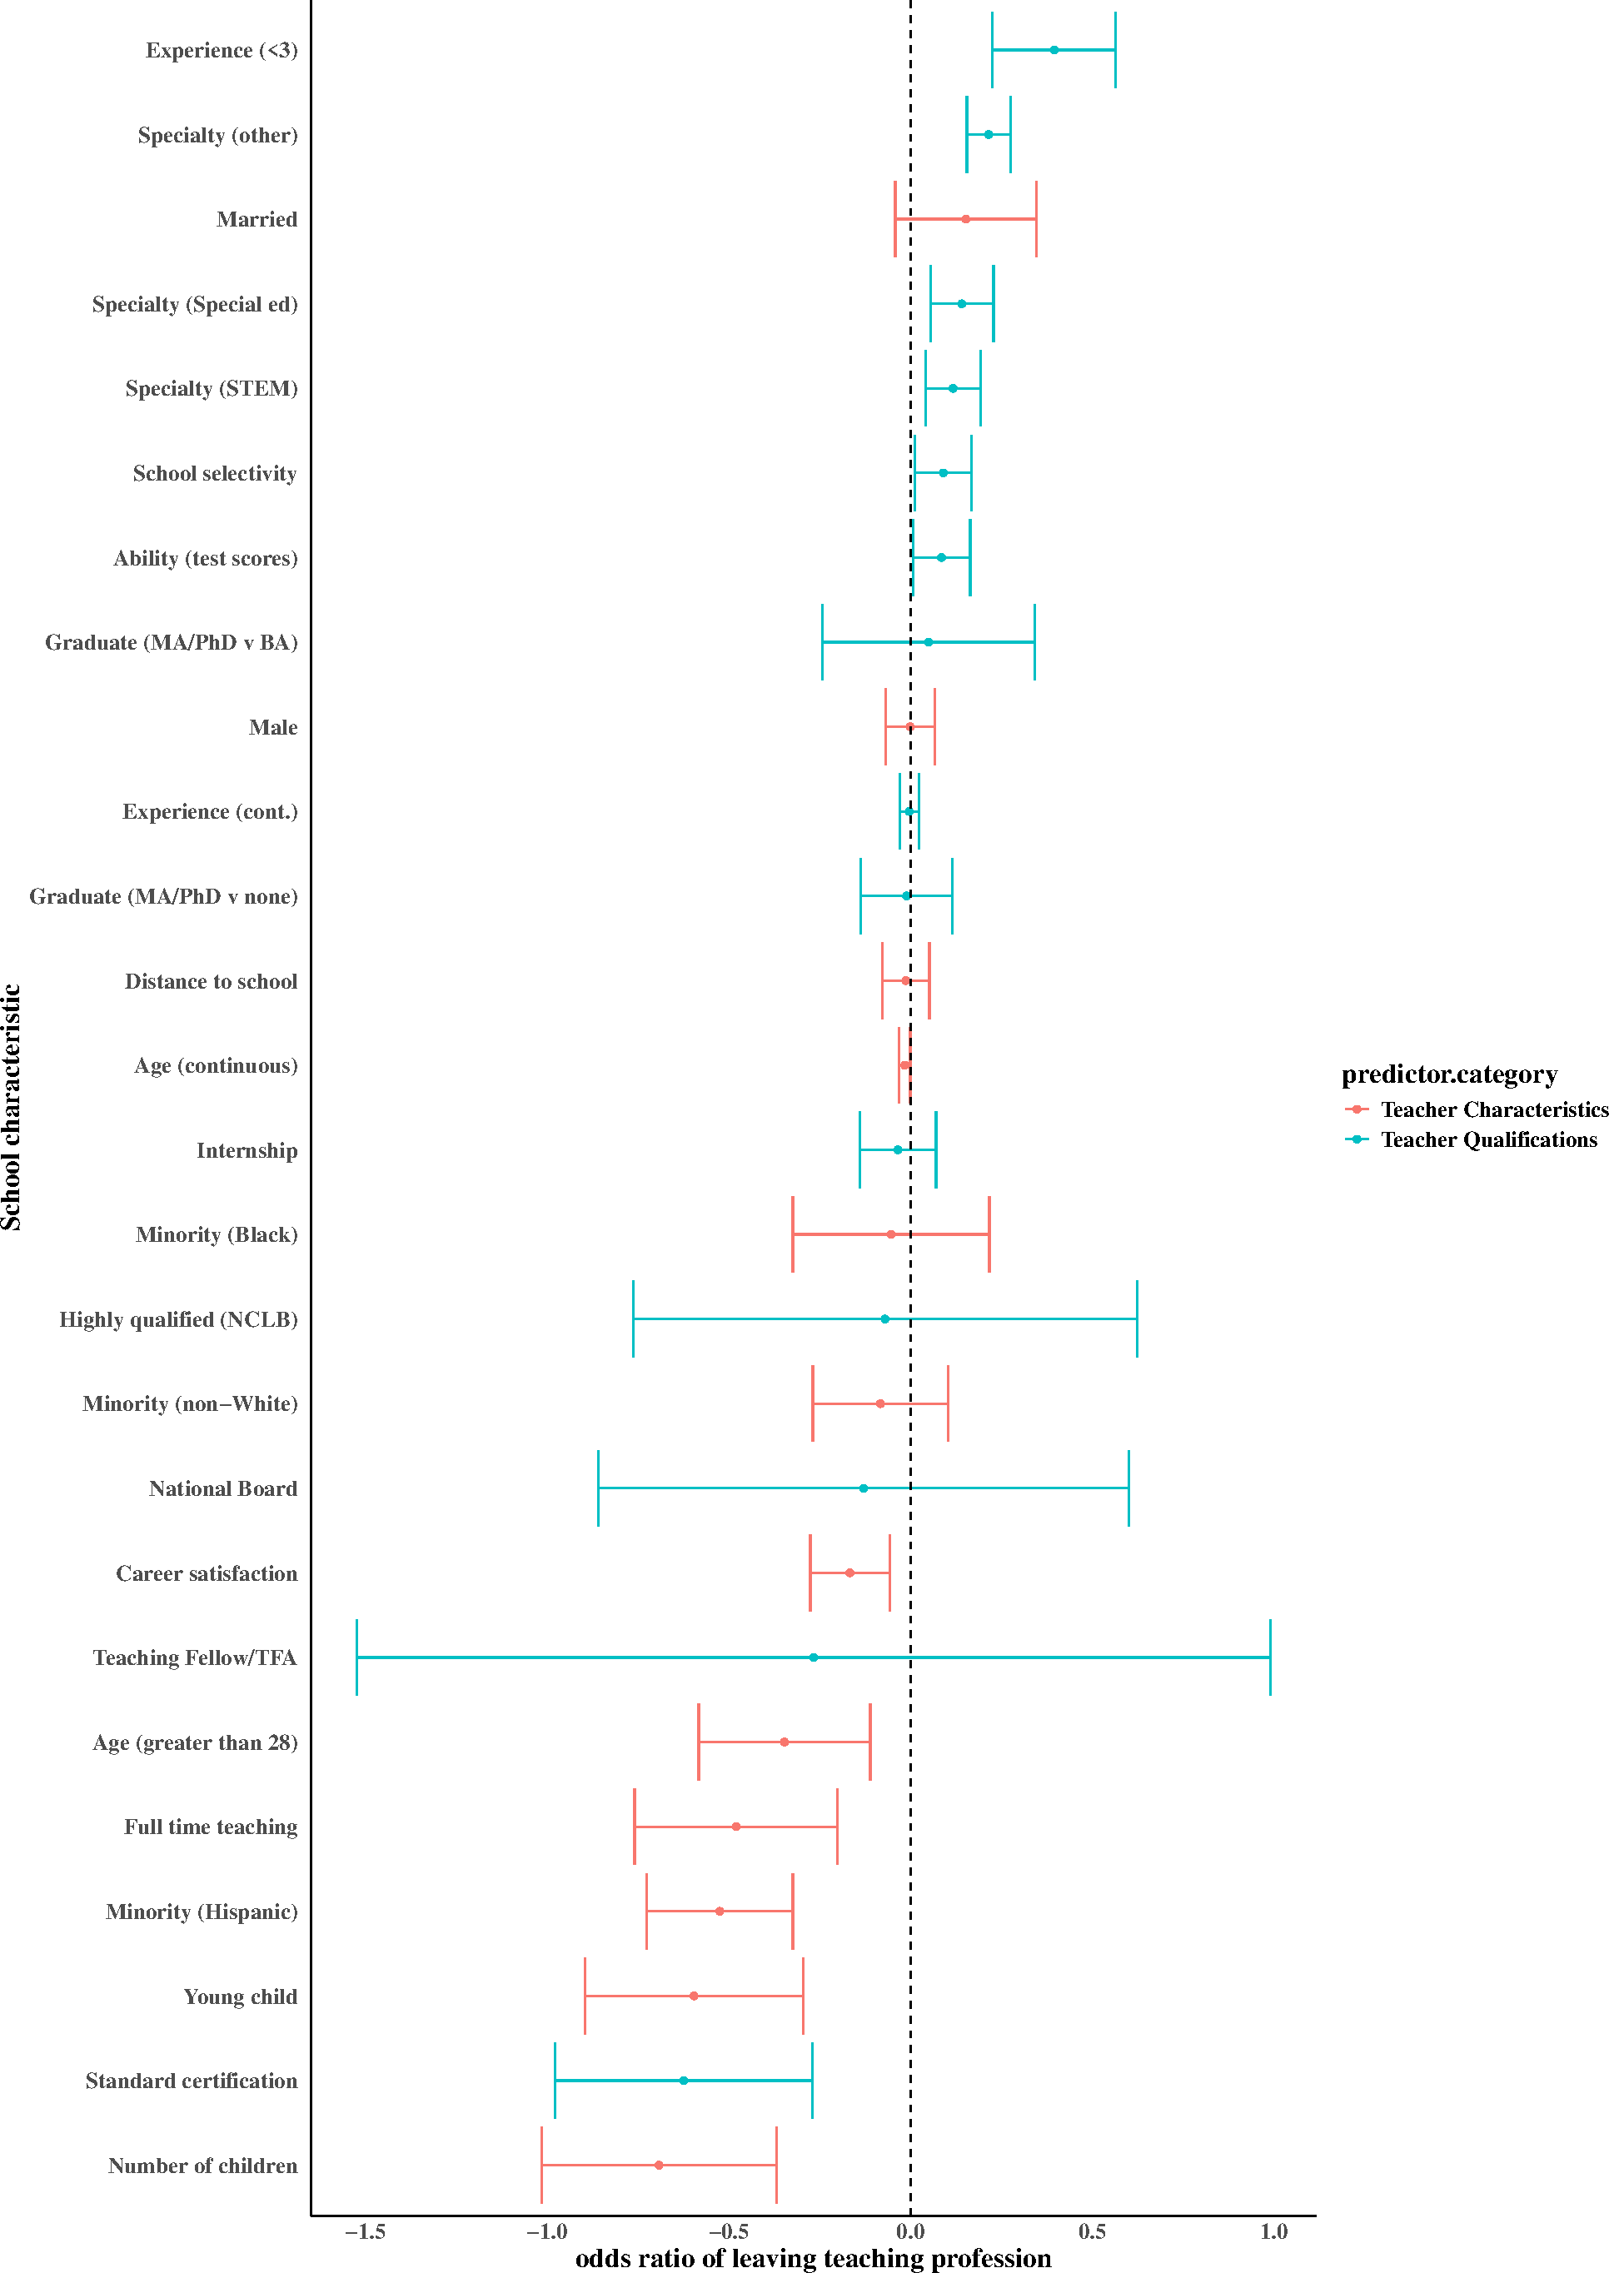
\includegraphics[width=1\linewidth,]{In-it-for-the-long-run_kollekolle_files/figure-latex/compare-effs-teacher-chars-1} \caption{Associations between leaving the teaching profession and teacher characteristics - reproduced from Nguyen, 2020}\label{fig:compare-effs-teacher-chars}
\end{figure}

As we can see, the scholarly literature suggests that there are a number of characteristics of both schools and teachers that impact the attrition and retention of teachers and, thereby, also the career choices of teachers. Interestingly, most student body characteristics and indicators of teacher ability are not among the most impactful of these characteristics. However, it should be noted that the results in Nguyen et al. (2020) pertain to leaving or staying in the current job, and not the entire career paths of teachers. As such, the results of Nguyen et al. (2020) cannot overrule choices in relation to the analysis of data that are founded in the theoretical framework of this paper.

\hypertarget{theory}{%
\section{Theory}\label{theory}}

In this paper, I chose to lean heavily on Carol Rinke's work as the basis of the theoretical framework. Rinke's work focuses on the dynamic process of how teachers shape their professional identity and how this process impacts teachers' career decisions.

\hypertarget{what-shapes-the-preferences-of-teachers}{%
\subsection{What shapes the preferences of teachers?}\label{what-shapes-the-preferences-of-teachers}}

Teachers' professional identity is likely to form the backbone of teachers' preferences towards the kind of school they want to work in or whether they'd prefer to opt out of teaching altogether. Teachers' professional identity comprises their aspirations, values, and how they explain their decisions and actions(Forde and McMahon 2019). Previous studies highlight the importance of teachers' understanding of themselves and how they use their professional identity to make sense of themselves as teachers. As such, teachers' professional identities likely guide how teachers make choices in terms of their careers, as well as how they relate to colleagues, students, and their everyday practice as teachers.(Rinke 2008)

Importantly, teachers' professional identities are not immutable but result from a dynamic process that constructs and alters their professional identity during their careers (Rinke 2014). Personal experience, professional practice, and the external environment all interact to shape teachers' professional identities. While some constituents of teachers' professional identity, e.g., experiences during childhood and adolescence, moral values, and experiences during education, are strong and lasting components of teachers' professional identity, other components, e.g.~professional practice, interactions with other teachers and students in different schooling context, are likely to contribute to the dynamic nature of teachers' professional identity(Rinke 2014). ``external'' factors, e.g., family formation, sickness, are also likely contributors to teachers' professional identity outside their experiences in schools(Attard Tonna and Calleja 2023)

As such, teachers' career choices can be seen as the \emph{enactment} of their professional identity.

\hypertarget{what-makes-some-schools-more-attractive-than-others}{%
\subsection{What makes some schools more attractive than others?}\label{what-makes-some-schools-more-attractive-than-others}}

The attractiveness of some schools, as opposed to others, is not arbitrary. This is highlighted in the work of (\textbf{Ingersoll\_2001?}), who points to the organizational features of schools as prominent ``push-and-pull'' factors for teachers.

The organizational features cover characteristics such as employee
compensation structure, administrative support, degree of conflict, and
strife, and employee influence over the organization
policies(\textbf{Ingersoll\_2001?}). Ingersoll's central premise is that these
factors impact, e.g., the cohesion among teachers and professional
motivation and thus influence how likely teachers are to stay at or
leave schools. Further, Ingersoll argues that schools faced with
external challenges, such as difficulties in hiring teachers due to being
located in a deprived neighborhood, are forced to decrease
organizational standards. For instance, principals facing trouble
attracting teachers specialized in teaching biology may assign teachers
with no specialization in biology to teach biology classes

Such organizational features are also present in Rinke's work and are often conceptualized as ``extrinsic factors.'' Rinke's study highlights that teachers actively evaluate their professional direction based on their identities and the alignment of their values with their work environment. For instance, teachers who feel a strong emotional connection to their workplace are more likely to remain in the profession, while those whose experiences contradict their ethical beliefs may choose to leave(Rinke and Mawhinney 2017)

\hypertarget{why-do-teachers-change-from-one-school-to-another}{%
\subsection{Why do teachers change from one school to another?}\label{why-do-teachers-change-from-one-school-to-another}}

The decision to leave one school in favor of another depends on the interplay between life experiences and the school context.

Working conditions and life experiences interact to form the picture of what success looks like to the teacher, and thus ultimately decide the career choice of the teacher(Rinke 2014). This choice, life experiences, and previous work experiences contribute to the ongoing construction of teachers' professional identities, which they will draw on to make future career decisions. In the framework of Rinke, this interaction is depicted as a process of negotiation, in which experiences in the workplace context are ``filtered'' by teachers' life experiences. Past experiences, e.g., personal and moral values, formative experiences during childhood and adolescence, and experiences throughout education and former workplaces, work as filters that aid the interpretation and management of experiences and challenges that teachers are exposed to in schools. It is in this negotiation between life experiences and experiences at the current workplace that teachers construct their perception of success(Rinke 2014)

As such, the decision to leave the current school in favor of another school occurs when the current perception of success does not align with the current work situation. One may imagine that a teacher aspires to make a difference for underprivileged students but is currently employed in a school of relatively affluent students. In such a situation, the current work context is not well aligned with the teachers' current perception of success.
In another situation, one may imagine a teacher with a background in STEM who has trouble sustaining themselves economically on a teacher's salary. At the same time, the teacher is disillusioned by feeling unprepared to teach primary school students and thus finds it very difficult to make the positive change the teacher had hoped to make when beginning a career as a teacher. In such a situation, the current perception of success would likely be to find employment in STEM for a higher salary and thus entirely leave teaching altogether.

\hypertarget{how-does-the-theory-predict-that-teachers-will-shape-their-career-paths}{%
\subsection{How does the theory predict that teachers will shape their career paths?}\label{how-does-the-theory-predict-that-teachers-will-shape-their-career-paths}}

Applying the theoretical framework of Rinke leads to a range of predicted findings.

\begin{itemize}
\item
  Career paths of teachers will vary between teachers due to the differences concerning professional identity
\item
  Teachers' career paths will exhibit dynamic patterns, i.e., teachers will switch between schools and different types of schools, e.g., between schools serving different kinds of student populations or opting in and out of teaching. This is to be expected due to the dynamic process that shapes teachers' professional identity throughout their careers. The propensity to switch between schools, types of schools, or opting in and out of teaching is also expected to vary between teachers
\item
  Teacher career paths will not be completely heterogeneous between teachers. Teachers who share experiences or who have had similar experiences, e.g., having had similar types of childhoods, or similar experiences within the educational system or sharing characteristics such as gender, ethnic origin, or geographic origin, will likely also share aspects of their professional identity. As such, it is expected that teachers with similar experiences or characteristics will have similar career paths, and these similarities in career paths can be used to construct a typology of teacher career paths.
\item
  Measurable characteristics of teachers will be associated with different types of career paths. While past experiences and personal characteristics feature prominently in Rinke's work, there are no precise and coherent descriptions of how certain experiences or characteristics would affect teacher career paths. Parts of her work, however, touch upon certain experiences and characteristics, chiefly the educational background and educational performance of teachers.

  \begin{itemize}
  \item
    Teachers' educational performance: In the work of Rinke, teachers with good educational performance or better/special credentials may show higher aspirations in terms of career. In particular, such teachers may have more employment opportunities outside teaching and thus be more inclined to leave teaching. As such, teachers with more opportunities outside teaching may also react more strongly to dissatisfactory work environments and may be more prone to switch to schools with better work environments or class environments where they can navigate more easily. As such, academically gifted teachers or have attained better credentials may be more prone to switch to schools with better resources or schools serving more affluent student populations if they do not opt out of teaching entirely(Rinke 2009). Additionally, the comparatively low perceived status of teaching may also push the most academically able teachers out of teaching. Even if the teachers themselves may prefer teaching due to, e.g.~moral values, teachers may not find support in their decision or even face resistance from their close ties who may purport the idea that academic ability is ``wasted'' on a career in teaching(Rinke 2014)
  \item
    Gender: The teacher's gender likely impacts their career decisions. Given that gender has likely been an influence on previous life experiences and is a part of the identity of teachers prior to their work as teachers, it is also likely that teachers' gender will exert an impact on their professional identity. However, the likely impact of gender on teachers' career decisions is unclear. Women face challenges in a number of professions due to gendered norms surrounding work, in which they are expected to, e.g., bear and care for children and bear the brunt of unpaid labor in the home. These gendered norms likely hold women back from participating in the labor market and professional advancement(Biklen 1995). Concerning gendered norms in teaching, these may work against men's decision to either choose or stay in teaching, as teaching is traditionally seen as a profession associated with women. In that sense, male teachers may feel a cultural deterrence to choose or stay in teaching, as they are expected to choose a career more aligned with classical views of male occupations(\emph{Opportunities and Challenges in Teacher Recruitment and Retention: Teachers' Voices Across the Pipeline} 2019).
  \item
    Geographic origin: While Rinke's work does not mention how geographic origin specifically impacts teachers' career decisions, it is mentioned as a part of the past experiences that shape teachers' professional identity. Previous studies have shown that teachers prefer to teach in close proximity to their geographic origin. As such, teachers originating from, e.g., rural areas are likely more prone to find employment in the types of schools found in such areas. Given that individuals with either high amounts of economic resources or those with college degrees tend to live in or around metropolitan areas, teachers from rural origins are likely less prone to be teaching in schools serving students with a high-SES background than teachers' from more urban or sub-urban origins.
  \end{itemize}
\end{itemize}

\begin{itemize}
\tightlist
\item
  Age: While most teachers' are similarly aged when they graduate, other teacher graduates may have opted into teaching from different occupations or educational tracks and will likely be older than their peers. Such teachers may have a more developed perception of success with regard to careers than their peers due to previous experiences in, e.g., the labor market or other educational tracks. As a result, these teachers may be more determined and motivated to make a career out of teaching than their younger peers, whose first experiences in the labor market will be as teachers.
\end{itemize}

\begin{itemize}
\tightlist
\item
  Marital status and children: Marriage and children are both events in teachers' personal lives that likely lead to a wish for more career stability. Married couples are likely to live or wish to live together, which means that decisions regarding residential location are now joint decisions of married couples. This likely restricts the geographic mobility of both individuals in the couple, which in turn restricts the choices of occupation in terms of geography. This restriction is further exacerbated by couples who are homeowners, as this adds additional economic restrictions, such as mortgage payments. Having children entails many of the same restrictions and demands for stability with respect to residential location. In addition, caring for children adds additional constraints on parents' time and economic resources. Additionally, marriage and family formation likely add a dimension of fulfillment in teachers' lives, which likely impacts teachers' perception of success in their careers, e.g., teachers may wish to balance career decisions such that future career decisions will lead to improvement in terms of work context but do not negatively impact either teachers' marriage or family, e.g., by having to relocate. As such, marriage and having children likely leads to more stable career patterns.
\end{itemize}

\hypertarget{data}{%
\section{Data}\label{data}}

In this paper, I use Danish administrative data covering two populations: all Danish primary school teachers from 1980 to 2020 and all Danish primary school students and their parents from 1980 to 2020.

In this paper, the population of teachers is further restricted. The population of Danish primary school teachers is restricted to only include teachers who graduated with a college degree in teaching in the years 1980-1985. There are two reasons for this restriction. Firstly, I chose to limit the years of graduation to the years 1980-1985, as this would allow me to investigate teacher careers over the course of 35 years while also yielding a population of considerable size as well as allowing me to investigate how teacher career paths vary between cohorts of teacher college graduates. Secondly, The population is restricted to only include teachers with a college degree in teaching. Career paths for teachers with a college degree in teaching have a natural starting point: the year that these teachers attained their degree in teaching. It is very hard to define a natural starting point for teachers who have not attained traditional qualifications as a teacher through a college degree. While one possible starting point might be the first job as a teacher, it is tough to precisely pinpoint when individuals were working as primary school teachers for the first time without having the entire labor market history of individuals. As data on labor market participation does not cover years earlier than 1980, it is very hard to precisely measure if individuals entered the labor market in 1980-1985, as the entire labor market history of most individuals in the labor market in 1980-1985 likely begins before 1980. I, therefore, chose to limit the population to teachers who had attained a college degree in teaching to work with a population that is well-defined and comprehensively covered in Danish administrative data.
In sum, the population of teachers in this paper covers teachers who graduated with a college degree in teaching between 1980 and 1985. The starting point of teachers' career sequences is defined by the year of graduation, and sequences extend to 35 years after graduation.

The population of students in primary schools from 1980 to 2020 and their parents is not restricted in any way. The data on students and their parents primarily serve to construct aggregated measures of students' SES background and educational attainment following primary school. Students are directly linked to schools in the Danish administrative data.

\hypertarget{linking-teachers-and-schools}{%
\subsection{Linking teachers and schools}\label{linking-teachers-and-schools}}

While the link between teachers and their workplaces is obtained directly from Statistics Denmark, the link between workplaces and primary schools needs to be constructed to link teachers to schools in which they are employed. To do this, public administrative data on all educational institutions(\url{https://data.stil.dk/instreghistorik/}) is linked to administrative data concerning teachers' workplaces via the ``unit of production'' identifier. The result is a combined dataset in which teachers are linked to the schools in which they are employed on a yearly basis through the link between teachers and their workplaces. The link between teachers' workplaces and primary schools is described in greater detail in Appendix XX

\hypertarget{teachers-career-sequences}{%
\subsection{Teachers' career sequences}\label{teachers-career-sequences}}

In this paper teachers career paths are comprised of sequences of career decisions, that are recorded on a yearly basis. Teachers career decisions are categorized into two primary categories: Working in different types of public primary schools or not working in public primary schools. These two primary categories are divided into different sub-categories, which are detailed below

\hypertarget{types-of-public-primary-schools}{%
\subsubsection{Types of public primary schools}\label{types-of-public-primary-schools}}

In this paper i will use the following school characteristics to construct a typology of schools.

\begin{itemize}
\tightlist
\item
  Average education of parents, at school level, measured in months
\item
  Average income of parents, at school level
\item
  Average high school enrollment rate: The proportion of students graduating in year \(t\) that are enrolled in high-school in year \(t+1\)
\end{itemize}

All school characteristics are time-varying, i.e.~averages have been computed for each school \(s\) in each year \(t\)

Parents educational level and income provide measurements of the average SES background of students at each school. The proportion of students enrolled in high school in the following provide an indirect measurement of student academic ability and academic aspirations. In the literature on teacher retention and attrition, both student SES background and academic ability prominently feature as factors that impact teachers' propensity to stay at or leave their current place of employment. For this reason, i expect that teachers will transition between schools vary on the chosen characteristics.

\hypertarget{constructing-school-types}{%
\subsubsection{Constructing school types}\label{constructing-school-types}}

In order to construct the different types of schools that teachers can be employed at, i aggregate the characteristics of each school in a linear scale, in which i scale and take the rowsum of the characteristics of each school, i.e.

\[School\ characteristics\ scale_{st}=\sum_{k=1}^{k}{school\ characteristics_{kst}}\]

All school characteristics are scaled within each year \(t\), i.e.~for each school characteristic, each value is scaled by the mean and standard deviation of the school characteristic within the current year instead of the mean and standard deviation across the entire sample. This is to avoid the scaling being dependent on trends in time that may be present for each of the characteristics. For instance, parental educational level increases quite dramatically from 1980-2020. On average, the average length of mothers education increased by nearly 3 years. As consequence, there would be very few schools in 1980 with a positive z-score on length of mothers education.

While this approach is simple compared to other approaches of constructing such a scale, e.g.~factor analysis or principal components analysis, performing a principal components analysis on the school characteristics suggests that the variables are correlated in highly unidimensional manner. In table \ref{tab:scale-qual} we see that the first principal component accounts for 72\% of the variance among the chosen school characteristics. As such, expanding the scale to include additional principal components would likely substantially increase complexity in order to account for a relatively small amount of variance.

\begin{table}[!h]
\centering
\caption{\label{tab:scale-qual}Summary of principal components analysis of school characteristics}
\centering
\begin{tabular}[t]{l|r|r|r|r|r}
\hline
  & PC1 & PC2 & PC3 & PC4 & PC5\\
\hline
Standard deviation & 1.90 & 0.96 & 0.54 & 0.34 & 0.25\\
\hline
Proportion of Variance & 0.72 & 0.18 & 0.06 & 0.02 & 0.01\\
\hline
Cumulative Proportion & 0.72 & 0.91 & 0.96 & 0.99 & 1.00\\
\hline
\end{tabular}
\end{table}

After having computed the scale-scores for each school, i then divide schools into 4 groups.

1: Schools that among the 0th and 25th percentile of the distribution of the ``school characteristics scale''

2: Schools that above the 25th percentile and at maximum the 50th percentile of the distribution of the ``school characteristics scale''

3: Schools that above the 50th percentile and at maximum the 75th percentile of the distribution of the ``school characteristics scale''

4: Schools that above the 75th percentile and at maximum the 100th percentile of the distribution of the ``school characteristics scale''

\hypertarget{career-decisions-outside-public-primary-schools}{%
\subsubsection{Career decisions outside public primary schools}\label{career-decisions-outside-public-primary-schools}}

In this paper, teachers are coded as working outside public primary schools if they cannot be linked to a public primary school through their workplace. Importantly, this does not mean that they do not work as primary school teacher or in other teaching positions. Teachers can work in private primary schools or in teaching positions in secondary education.

\hypertarget{teacher-characteristics}{%
\subsection{Teacher characteristics}\label{teacher-characteristics}}

In addition to investigating the distribution of teachers' career sequences, i will also investigate whether characteristics of teachers are associated with the different types of teacher career sequences.

Following the theoretical framework i will include the following teacher characteristics as predictors of membership in types of teacher career sequences.

Teachers' gender: A binary variable indicating whether teachers are registered as female or male in the danish administrative data

Teachers' high-school GPA: A continuous variable measuring the overall high-school GPA of teachers. While it would have been more relevant to include the teachers' college GPA, teachers' college GPA is covered in the danish administrative data earlier than 2004.

Number of children in household: A continuous, integer-valued, variable measuring the number of children living in the household of the teacher

Teachers' marital status: A discrete variable indicating whether teachers are unmarried, married or divorced.

Type of municipality: A discrete variable indicating whether the teacher lived in one of five types of municipality

\begin{enumerate}
\def\labelenumi{\arabic{enumi})}
\item
  Municipalities in the capital region
\item
  Municipalities in metropolitan areas
\item
  Municipalities in suburban areas
\item
  Municipalities in provincial areas
\item
  Municipalities in rural areas
\end{enumerate}

Age at graduation: A continuous, integer-valued, variable measuring the age of teachers, in years, at the time teachers attained their college degree in teaching

Year of graduation: A discrete variable indicating in which year the teacher graduated

all covariates are measured at the time of graduation, and are thus time-invariant. As such, teacher marital status may change during the course of teachers' careers, but in this paper teachers' marital status indicates the marital status of teachers in the same year that they attained their college degree in teaching. This choice may seem overly restrictive, but it is not trivial to include time-varying covariates in sequence analysis

\hypertarget{methods}{%
\section{Methods}\label{methods}}

\hypertarget{sequence-analysis}{%
\subsection{Sequence analysis}\label{sequence-analysis}}

In this paper i will investigate sequences of teacher career decisions using sequence analysis. Sequence analysis aims to apply a more holistic approach to e.g.~analysis of career decisions or transitions between life course events such as marriage, family formation etc., as opposed to e.g.~regression approaches that aim to model the average probability of transition between one state to another. As such, sequence analysis is also a more descriptive technique. In this paper i will primarily use sequence analysis for three purposes.

\begin{enumerate}
\def\labelenumi{\arabic{enumi})}
\item
  Investigating the overall distribution of teacher carer sequences
\item
  Constructing a typology of teacher careers by applying optimal matching and cluster analysis to teacher sequences
\item
  Investigating associations between teacher characteristics and membership of teacher career types
\end{enumerate}

I will use the R package ``TraMineR'' to carry out much of the analysis

\hypertarget{distribution-of-sequences}{%
\subsubsection{Distribution of sequences}\label{distribution-of-sequences}}

In this paper sequences of teacher career decisions are constructed as consecutive teacher career, during the years 1-35 since graduation, decisions within the state space defined by the data. For instance a sequence of career decision in the first 5 years since graduation may look like \emph{school type 1-\textgreater school type 1-\textgreater school type 1-\textgreater private school-\textgreater private school} for one teacher and may look like \emph{school type 1-\textgreater school type 2-\textgreater school type 2-\textgreater school type 4-\textgreater school type 4} for another teacher. Taken together across all teachers we get a distribution of sequences, where we can asses the share of teachers in each type of career decision across years since graduation, e.g.~in year 2 since graduation, 10\% of teachers may be employed in school type 1 and 8\% are employed in private schools, while in year 3 since graduation 7\% of teachers may be employed in school type 1 and 11\% are employed in private schools.

\hypertarget{how-will-sequences-be-clustered}{%
\section{How will sequences be clustered?}\label{how-will-sequences-be-clustered}}

After having constructed the sequences, i will investigate if similar sequences can be clustered together to form different types of career sequences. To do this i will:

\begin{enumerate}
\def\labelenumi{\arabic{enumi})}
\item
  Measure the similarity between sequences of teacher career sequences, using ``optimal matching''(REF Abbot)
\item
  Use hierarchical clustering to construct types of career sequences. Additionally i will use range of statistics describing the ``fit'' of the clustering procedure when the number of clusters vary. This is a data-driven procedure that aims to aid in deciding which number of clusters will lead to the ``optimal'' clustering of similar sequences of career decisions.
\end{enumerate}

\hypertarget{sequence-similarity}{%
\subsection{sequence similarity}\label{sequence-similarity}}

The similarity of sequences is measured using optimal matching. Optimal matching attempts to align sequences such that they are identical using 3 different operations: Substitution, insertion and deletion. For each of these operations a ``cost'' assigned, which will ultimately determine how similar sequences are measured to be, following the optimal matching procedure. As an example we can see optimal matching would determine the similarity of the two previous sequences.

Sequence 1: school type 1 -\textgreater{} school type 1 -\textgreater{} school type 1 -\textgreater{} private school -\textgreater{} private school

Sequence 2: school type 1 -\textgreater{} school type 2 -\textgreater{} school type 2 -\textgreater{} school type 4 -\textgreater{} school type 4

In this case 4 operations would be needed to align the sequences:

1: substitute the second element in sequence 1, school type 1, for school type 2

2: substitute the third element in sequence 1, school type 1, for school type 2 '

3: substitute the fourth element in sequence 1, private school, for school type 4

4: substitute the fifth element in sequence 1, private school, for school type 4

As such, the distance between sequence 1 and 2 is four operations according to OM

In the example above either of the three operations had the same ``cost'', which was 1. However insertions and deletions can be more or less costly than substitutions and not all substitutions need to have the same cost. For instance substituting school type 4 for school type 1 can be more costly than substituting school type 1 for school type 4.

The costs for for substitutions,deletions and insertions can be set by the user following e.g.~theoretical considerations. In this paper however, i have chosen a data-driven strategy for setting these costs, by relying on the inverse of the observed transition rates between states. As such, the substitution costs between states is given by

\(SC(i,j) = cval - P(i|j) -P(j|i)\)

Where \(i\) and \(j\) represent states, while \(P(i|j)\) and \(P(j|i)\) is the probability of transitioning from state \(i\) to \(j\) and from state \(j\) to \(i\) respectively. \(cval\) is a constant with the value of 2

In table \ref{tab:trate} the observed transition probabilities between states is shown, and in table \ref{tab:cost} the cost associated with each type of substitution is shown. The insertion and deletion costs are both 1.

\begin{table}

\caption{\label{tab:trate}Transition rates between states}
\centering
\begin{tabular}[t]{l|r|r|r|r|r}
\hline
  & [Not teacher ] & [0-25\% ] & [>50\%-75\% ] & [>25\%-50\% ] & [>75\%-100\% ]\\
\hline
[Not teacher ->] & 0.94 & 0.02 & 0.01 & 0.01 & 0.01\\
\hline
[0-25\% ->] & 0.06 & 0.78 & 0.02 & 0.14 & 0.01\\
\hline
[>50\%-75\% ->] & 0.05 & 0.01 & 0.71 & 0.13 & 0.09\\
\hline
[>25\%-50\% ->] & 0.06 & 0.13 & 0.13 & 0.67 & 0.01\\
\hline
[>75\%-100\% ->] & 0.05 & 0.01 & 0.10 & 0.01 & 0.83\\
\hline
\end{tabular}
\end{table}

\begin{table}

\caption{\label{tab:cost}Substitution costs between states}
\centering
\begin{tabular}[t]{l|r|r|r|r|r}
\hline
  & Not teacher & 0-25\% & >50\%-75\% & >25\%-50\% & >75\%-100\%\\
\hline
Not teacher & 0.00 & 1.92 & 1.94 & 1.93 & 1.94\\
\hline
0-25\% & 1.92 & 0.00 & 1.97 & 1.73 & 1.99\\
\hline
>50\%-75\% & 1.94 & 1.97 & 0.00 & 1.73 & 1.80\\
\hline
>25\%-50\% & 1.93 & 1.73 & 1.73 & 0.00 & 1.98\\
\hline
>75\%-100\% & 1.94 & 1.99 & 1.80 & 1.98 & 0.00\\
\hline
\end{tabular}
\end{table}

\hypertarget{hierarchical-clustering}{%
\subsection{Hierarchical clustering}\label{hierarchical-clustering}}

Hierarchical clustering is a method used to group similar sequences into clusters based on their dissimilarity. It builds a hierarchy or a tree of clusters, known as a dendrogram, which can be cut at different levels to form various numbers of clusters.

Briefly, hierarchical clustering iterates by merging observations into clusters until all observations belong to one single cluster. The process is depicted in figure \ref{fig:clus-ex}. In this paper i have chosen to use Wards method as the linkage criterion.

\begin{figure}[H]
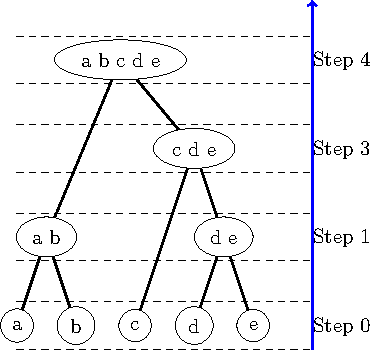
\includegraphics{In-it-for-the-long-run_kollekolle_files/figure-latex/clus-ex-1} \caption{adapted from http://www.sthda.com/sthda/RDoc/images/hierarchical-clustering-agnes-diana.png}\label{fig:clus-ex}
\end{figure}

\hypertarget{determining-optimal-number-of-clusters}{%
\subsubsection{Determining optimal number of clusters}\label{determining-optimal-number-of-clusters}}

As shown in figure \ref{fig:clus-ex}, the clustering process continues until all individual sequences are clustered into a single cluster, but it does not suggest at which step, the optimal clustering of sequences has been achieved. While, there is no clear consensus on how one decides which number of clusters will be ``optimal'' there are several measures that can aid the decision. In this paper i have chosen to apply the average silhouette width(ASW) as a measure of fit across solutions with different numbers of clusters, as this measure has several favorable properties. The silhouette width of each sequence can be though of a measure of well each sequence fits into the cluster to which it is assigned. Positive values of silhouette width indicates that a given sequence fits better into the cluster to which it is assigned than to the nearest ``neighboring'' cluster, i.e.~the cluster in which the sequence would have the second best fit. Conversely, a negative value silhouette width indicates that the given sequence would actually fit better in the nearest neighboring cluster than the one to which it is currently assigned(Studer 2013).

\hypertarget{predicting-cluster-membership-using-teacher-characteristics}{%
\subsection{Predicting cluster membership using teacher characteristics}\label{predicting-cluster-membership-using-teacher-characteristics}}

In this paper i will investigate the association between a range of teacher characteristics and the types of career paths that teachers are assigned to via the clustering procedure. In order to account for unspecified non-linear functional forms, interactions between predictors or other deviations constraints of classical regression frameworks, e.g.~linearity in parameters, i will apply flexible machine learning (ML) techniques. Many of these techniques are known to ``learn'' the functional form of associations between outcomes and predictors from data. Additionally tree-based techniques, such as decision trees, random forests and gradient boosted trees, are known to also learn unspecified interactions between predictors. I will also compare the predictive performance of the ML techniques with the performance of multinomial regression, which is the traditional estimation technique used to investigate relations between predictors and typologies of sequences.

I will use the following approaches to investigate the associations between teacher characteristics and types of career sequences:

\begin{itemize}
\item
  Multinomial logistic regression, implemented via the function ``multinom'' from the package ``nnet'' in R
\item
  Elastic net regression: Elastic net regression is a type of penalized regression, where regression coefficients are ``penalized'' according to an amount specified by the user. Elastic net combines both L1- and L2-penalization according to a ``mixing weight'' which controls the proportion of penalization that is attributed to either L1 or L2 penalization. Elastic Net can handle scenarios with highly correlated features and can perform better than linear regression by reducing overfitting and improving generalization. Elastic net is implemented via the ``glmnet'' package in R
\item
  Decision Tree:
  A decision tree is a flowchart-like model that splits data into subsets based on variable values, leading to a tree structure. RPART (Recursive Partitioning and Regression Trees) is an implementation in R.
  Decision trees can capture non-linear relationships and interactions between features, regardless of whether these are specified or not. While this ability of decision trees is not guaranteed to automatically find the true functional form of relationships or all interactions between variables, this ability may still lead to improvements over multinomial regression.Decision trees are implmented via the ``rpart'' package in R
\item
  Conditional Inference Tree (ctree):
  A conditional inference tree is a type of decision tree that uses statistical tests to select splits rather than greedy algorithms. It controls for overfitting by stopping the tree when splits are not statistically significant.
  By focusing on statistically significant splits, ctrees reduce the risk of overfitting and can model complex interactions. This may be an improvement over traditional implementations of decision trees, which are prone to overfitting.
\item
  Support Vector Machine (SVM):
  SVM is a classification and regression algorithm that finds the hyperplane that best separates data points into different classes. It can handle both linear and non-linear data using kernel functions.
  SVM is particularly effective in high-dimensional spaces and can capture complex, non-linear relationships, offering better performance in cases where linear regression would be insufficient. SVM has proven highly effective in other practical applications.
\item
  K-Nearest Neighbors (KNN):
  KNN is a simple, non-parametric algorithm that predicts the outcome by averaging the values of the k nearest data points in the feature space.
  KNN can model non-linear relationships without making assumptions about the data distribution, potentially outperforming multinomial regression, especially in cases with complex patterns.
\item
  Multivariate Adaptive Regression Splines(MARS):
  Known as MARS, this method builds flexible models by creating piecewise linear regressions over different intervals of the data. Similar to decision trees, MARS has the ability to capture unspecified interactions between variables. MARS is a regression approach at its core however, and may therefore be better suited to model continous predictors than decision trees. MARS is implemented via the ``earth'' package in R.
\item
  Gradient Boosted Trees (GBM):
  GBM is an ensemble technique that builds multiple decision trees sequentially, each trying to correct the errors of the previous ones.
  GBM can model intricate patterns and interactions in the data by combining the strengths of multiple weak learners (decision trees). As such, gradient boosted trees improve upon approaches that use a single decision tree.
\item
  Extreme Gradient Boosting (XGBoost):
  XGBoost is an optimized implementation of gradient boosting that is highly efficient, flexible, and portable, often used in machine learning competitions. XGboost is an extension upon GBM, which is intitially due it's optimized implementation, which reduces computing time. However XGboost also features other extensions, e.g.~additional hyperparameters, that may lead to better predictive performance.
\item
  Random Forest:
  Random Forest is an ensemble learning method that builds multiple decision trees and combines their predictions to improve accuracy and control overfitting.
  By averaging the predictions from various decision trees, Random Forest reduces variance, can handle large datasets with higher dimensionality, and can capture non-linear relationships. While random forests are initially an improvement upon single decision trees, random forests have shown to deliver good predictive performance even when compared with more advanced machine learning techniques, such as GBM and XGboost.
\end{itemize}

For further information on either of the ML techniques readers are referred to (James et al. 2021)

In order to asses the predictive performance and find the optimal combination of hyperparameter configurations for each ML technique i apply repeated K-fold cross-validation(CV). Briefly, CVinvolves splitting data into K partitions, usually denoted ``folds'', where each partition divides the full data into ``training'' and ``testing'' parts. The model is then fitted on the training portion of the data and the fitted model is then used to predict the outcome in the test-portion of the data, as depicted in figure \ref{fig:cv-figure}. CV, or similar procedures, are crucial when assessing the predictive performance of ML techniques. For many of these techniques, the flexibility and complexity can be substantial and the techniques may overfit to data as a result, which skews measures of predictive performance in a positive direction. As such, CV functions as a general and non-parametric way of giving an unbiased estimate of predictive performance(James et al. 2021). In that sense CV also serves as a standardized way of comparing techniques for which the internal workings differ greatly. In my application i use 10-fold CV, which is repeated 2 times.

\begin{figure}[H]
\includegraphics{In-it-for-the-long-run_kollekolle_files/figure-latex/cv-figure-1} \caption{Depiction of 5-fold CV}\label{fig:cv-figure}
\end{figure}

Many of the ML techniques have several hyperparameters that impact the predictive performance, e.g.~the degree of penalization of elastic net or the number of trees to aggregate in random forest. To pick the optimal combination of these hyperparameters for each technique, each technique will be fit, using CV, on a range of hyperparameter combinations. The hyperparameter combination with the best predictive performance will then be chosen. For models with few adjustable hyperparameters i will use a ``grid search'' in which all combinations of chosen hyperparameter-values are assessed. For techniques with more adjustable hyperparameters, in this case GBM, XGBoost and random forest, i will pick 200 random hyperparameter combinations. Using random hyperparameter combinations is often a effective way to cover the search space of hyperparameter combinations, as opposed to doing a grid search which quickly results in thousands of hyperparameter combinations to asses in order to cover the hyperparameter search space adequately(Bergstra and Bengio 2012)

To measure the predictive performance i will use Cohens Kappa, which is given by

\begin{equation} 
  \kappa=\frac{p_0-p_t}{1-p_t}
  \label{eq:kappa}
\end{equation}

In which \(p_0\) is the proportion of agreements between predictions and observed values, while \(p_t\) is the hypothetical proportion of agreement between predictions and observed values purely by chance. The kappa value ranges between 0 and 1, where 0 indicates that predictions and observed values are in no better agreement than what could be expected by chance. I have chosen Cohens Kappa as a measure of predictive performance, given that this measure is robust to ``class imbalance'', i.e.~some categories of the outcome being much more prevalent than others. For instance, if the typology of career sequences is dominated by a single type in which 90\% of teachers are assigned, then it would be easy to get 90\% of predictions correct simply by predicting all teachers to be in the most prevalent type. The kappa value is robust to such a situation however

Cross-validation and fitting of all ML techniques were implemented using the ``caret'' package in R

\hypertarget{imputing-school-characteristics}{%
\section{Imputing school characteristics}\label{imputing-school-characteristics}}

Data on the school characteristics that comprise the scale used to construct the types of schools are in many cases
plagued by missing data. This complicates analysis, as school types then cannot be determined for some schools, in some years. To alleviate this issue, i opted to impute data on school characteristics using linear regression. Data is imputed by fitting a model in which the school characteristic in question is predicted by an indicator for year and school fixed effects, to account for variance between schools. To accommodate for a non-linear time trend, the relation between \(year_s\) and \(School\ characteristic_{st}\) is fitted using a 5th degree polynomial and a school fixed effect, \(\alpha_s\).

\(School\ characteristic_{st}=\beta_0+\beta_1 year_{t}+\beta_2 year^2_{t}+\beta_3 year^3_{t}+\beta_4 year^3_{t}+\beta_5 year^4_{t}+\beta_6 year^5_{t}+\alpha_s\)

\hypertarget{results}{%
\section{Results}\label{results}}

\hypertarget{descriptive-statistics}{%
\subsection{Descriptive statistics}\label{descriptive-statistics}}

In the following i will present descriptive statistics for both teachers and the types of schools

\hypertarget{teachers}{%
\subsubsection{Teachers}\label{teachers}}

In table \ref{tab:des-teach}, descriptive statistics are presented for teachers in the first year since graduation. Statistics are presented across teacher ``cohorts'', which indicate the year at which each cohort graduated from teacher college.
The majority of teachers are unmarried, female and do not have any children. Further, nearly all teachers are from the ethnic majority.

\setlength{\LTpost}{0mm}
\begin{longtable}{p{3cm}p{1.5cm}p{1.5cm}p{1.5cm}p{1.5cm}p{1.5cm}p{1.5cm}p{1.5cm}}
\caption{Descriptive statistics for teachers}
    \label{tab:des-teach}\\
\toprule
\textbf{Characteristic} & \textbf{Overall}, N = 13,283\textsuperscript{\textit{1}} & \textbf{1980}, N = 2,533\textsuperscript{\textit{1}} & \textbf{1981}, N = 2,382\textsuperscript{\textit{1}} & \textbf{1982}, N = 2,342\textsuperscript{\textit{1}} & \textbf{1983}, N = 2,208\textsuperscript{\textit{1}} & \textbf{1984}, N = 2,114\textsuperscript{\textit{1}} & \textbf{1985}, N = 1,704\textsuperscript{\textit{1}} \\ 
\midrule\addlinespace[2.5pt]
age & 29 (5) & 29 (5) & 29 (5) & 29 (5) & 29 (5) & 29 (5) & 29 (5) \\ 
unmarried & 7,596 (57\%) & 1,303 (51\%) & 1,285 (54\%) & 1,291 (55\%) & 1,292 (59\%) & 1,311 (62\%) & 1,114 (65\%) \\ 
female & 7,770 (58\%) & 1,413 (56\%) & 1,350 (57\%) & 1,368 (58\%) & 1,280 (58\%) & 1,295 (61\%) & 1,064 (62\%) \\ 
number of children in household & 0.70 (2.25) & NA (NA) & NA (NA) & NA (NA) & NA (NA) & 0.75 (2.91) & 0.64 (0.90) \\ 
Unknown & 9,465 & 2,533 & 2,382 & 2,342 & 2,208 & 0 & 0 \\ 
Ethnic minority status &  &  &  &  &  &  &  \\ 
Born in Denmark & 13,089 (99\%) & 2,501 (99\%) & 2,335 (98\%) & 2,304 (98\%) & 2,181 (99\%) & 2,088 (99\%) & 1,680 (99\%) \\ 
Immigrant & 152 (1.1\%) & 26 (1.0\%) & 37 (1.6\%) & 28 (1.2\%) & 19 (0.9\%) & 23 (1.1\%) & 19 (1.1\%) \\ 
1st generation descendant of immigrants & 42 (0.3\%) & 6 (0.2\%) & 10 (0.4\%) & 10 (0.4\%) & 8 (0.4\%) & 3 (0.1\%) & 5 (0.3\%) \\ 
\bottomrule
\end{longtable}
\begin{minipage}{\linewidth}
\textsuperscript{\textit{1}}Mean (SD); n (\%)\\
\end{minipage}

\hypertarget{schools}{%
\subsubsection{Schools}\label{schools}}

In table \ref{tab:des-schools} i present descriptive results for the different types of schools. The average score of the school characteristics scale for each school type is reported in the bottom row. Here we can clearly see how school characteristics vary across school-types, with schools above the 75th percentile of the school characteristics scale having more than 20 months of additional education, compared to schools between the 0th and 25th percentile, for both mothers and fathers. The pattern is similar for the remaining school characteristics.

\setlength{\LTpost}{0mm}
\begin{longtable}{lcccc}
\caption{Descriptive statistics for schools}
    \label{tab:des-schools}\\
\toprule
\textbf{Characteristic} & \textbf{0-25\%}, N = 50,989\textsuperscript{\textit{1}} & \textbf{\textgreater{}25\%-50\%}, N = 54,236\textsuperscript{\textit{1}} & \textbf{\textgreater{}50\%-75\%}, N = 57,575\textsuperscript{\textit{1}} & \textbf{\textgreater{}75\%-100\%}, N = 52,460\textsuperscript{\textit{1}} \\ 
\midrule\addlinespace[2.5pt]
Average length of mothers education, in months & 145 (14) & 153 (12) & 157 (12) & 168 (13) \\ 
Average length of fathers education, in months & 150 (10) & 157 (8) & 162 (8) & 173 (10) \\ 
Average yearly disposable income of mothers in DKK & 139,876 (64,018) & 155,764 (63,249) & 156,520 (68,833) & 181,759 (92,592) \\ 
Average yearly disposable income of fathers in DKK & 146,979 (70,284) & 175,305 (71,828) & 184,225 (79,791) & 236,917 (139,759) \\ 
Proportion of students enrolled in secondary education the following year & 0.18 (0.08) & 0.22 (0.07) & 0.26 (0.08) & 0.37 (0.13) \\ 
Unknown & 131 & 81 & 166 & 11 \\ 
Proportion of students who are immigrants or descendants of immigrants & 0.15 (0.19) & 0.08 (0.10) & 0.06 (0.07) & 0.05 (0.06) \\ 
Avg. high school GPA of teachers & 79 (8) & 79 (8) & 80 (8) & 80 (8) \\ 
Unknown & 36,180 & 38,215 & 42,453 & 39,106 \\ 
Z-score of summed school characteristics & -4.4 (1.6) & -1.6 (0.6) & 0.6 (0.7) & 5.2 (3.4) \\ 
\bottomrule
\end{longtable}
\begin{minipage}{\linewidth}
\textsuperscript{\textit{1}}Mean (SD)\\
\end{minipage}

\hypertarget{sequence-analysis-1}{%
\subsection{Sequence analysis}\label{sequence-analysis-1}}

In figure \ref{fig:overall-seq-plot} we see the overall distribution of sequences for all teachers. While it is not surprising that the four different types of schools occupy roughly equal proportions of teacher career choices in each year, it is somewhat surprising that the proportion of teacher graduates that are not working in a public primary school is very high. While the proportions of teachers outside public primary schools continues to decrease until the very late stages of teacher careers, the proportion is consistently above 50\% of teachers until the late stages of teacher career paths.

\begin{figure}[H]
\includegraphics{In-it-for-the-long-run_kollekolle_files/figure-latex/overall-seq-plot-1} \caption{overall distribution of sequences}\label{fig:overall-seq-plot}
\end{figure}

\hypertarget{clustering-sequences}{%
\subsubsection{Clustering sequences}\label{clustering-sequences}}

In the following section i will investigate how teacher career trajectories can be separated into different types of career trajectories using cluster analysis using the procedures described in the \emph{methods} section. As described i will use the ASW measure to select the optimal number of clusters.

In table \ref{tab:cluster-choice} we see that the ASW measure favors a solution with four clusters

\begin{table}[!h]
\centering
\caption{\label{tab:cluster-choice}optimal number of clusters across measures}
\centering
\begin{tabular}[t]{l|r|r|r|r|r|r|r|r|r|r}
\hline
  & PBC & HG & HGSD & ASW & ASWw & CH & R2 & CHsq & R2sq & HC\\
\hline
2 clusters & 0.59 & 0.68 & 0.68 & 0.39 & 0.39 & 4660.02 & 0.25 & 8877.64 & 0.39 & 0.15\\
\hline
3 clusters & 0.70 & 0.82 & 0.82 & 0.40 & 0.40 & 3250.28 & 0.32 & 7150.73 & 0.50 & 0.08\\
\hline
4 clusters & 0.75 & 0.90 & 0.90 & 0.42 & 0.42 & 2868.40 & 0.38 & 7119.42 & 0.60 & 0.05\\
\hline
5 clusters & 0.61 & 0.79 & 0.79 & 0.32 & 0.32 & 2701.91 & 0.43 & 6456.15 & 0.65 & 0.11\\
\hline
6 clusters & 0.63 & 0.83 & 0.83 & 0.32 & 0.32 & 2440.55 & 0.46 & 6253.28 & 0.69 & 0.09\\
\hline
7 clusters & 0.58 & 0.83 & 0.83 & 0.30 & 0.30 & 2204.07 & 0.48 & 5668.61 & 0.71 & 0.10\\
\hline
\end{tabular}
\end{table}

In figure \ref{fig:cluster-seq-plot} we see the distributions of sequences across each of the four clusters. Following figure \ref{fig:overall-seq-plot} it is perhaps not surprising to see that the decision to not work in a public primary school features prominently. However in figure \ref{fig:cluster-seq-plot} we see that the decision to not work in public primary school features heavily in a large group of teacher graduates who only rarely work in any type of public primary school, during their entire career. The two smallest clusters, cluster 2 and cluster 3 contrast each other, given that the majority if teachers in cluster 3 work at schools in upper end of the distribution of the school characteristics scale, while the opposite is true of teacher in cluster 2. Interestingly, teachers in cluster 3 are more homogeneous in their choice of school, than teachers in cluster 2. While teachers in cluster 2, in contrast work in the least advantaged schools they also work in the schools between the \textgreater25th percentile and 50th percentile. The last cluster, cluster 4, is more balanced, although the majority of teachers work in the ``middle range'' of school types.
While the proportion of teachers working outside public primary schools is similar in clusters 3 and 4, this proportion is generally larger for teachers in cluster 2, in the early career of teachers.

\begin{figure}[H]
\includegraphics{In-it-for-the-long-run_kollekolle_files/figure-latex/cluster-seq-plot-1} \caption{distribution of sequences across clusters}\label{fig:cluster-seq-plot}
\end{figure}

\hypertarget{predicting-clusters}{%
\subsection{Predicting clusters}\label{predicting-clusters}}

In this section i will present the predictive performance of the different ML techniques. Next i will present a measure of variable importance of the best performing ML technique, and choose the 3 most important variables for further interpretations. To further investigate the association between the 3 most important variables and cluster membership, i will present these associations using ``partial dependence plots''.

In addition to the teacher characteristics detailed in the \emph{data} section of this paper, i also include two measures of ``misclassification'' with regards to cluster membership. I include the silhouette width for each observation, which, as described, represents a measure of how well each career sequence fits within the assigned cluster compared to the ``nearest neighbor'' cluster. I also include an indicator for which cluster is the nearest neighbor. I include these to account for correlation between misclassification and teacher characteristics.

\hypertarget{performance-of-ml-models}{%
\subsubsection{Performance of ML models}\label{performance-of-ml-models}}

In figure \ref{fig:ml-perf} we see that GBM achieved the highest performance, although the predictive performance of GBM is close to that of other tree-based techniques. While the performance of GBM is better than techniques based on linear regression, the differences in kappa-values are not large. While the 1st quartile of GBM is higher than the 3rd quartile of multinomial regression, this is not true when comparing to the performance of elastic net.

\begin{figure}[H]
\includegraphics{In-it-for-the-long-run_kollekolle_files/figure-latex/ml-perf-1} \caption{predictive performance of ML techniques}\label{fig:ml-perf}
\end{figure}

\hypertarget{variable-importance}{%
\subsection{Variable importance}\label{variable-importance}}

In this section i will investigate the strength of the association between the included variables and cluster membership. While predictive performance was generally good for the best performing techniques, measures of variable importance suggest that measures of misclassification were far more predictive of cluster membership than teacher characteristics. Variable importance measures of advanced ML techniques are generally hard to interpret. I therefore use the predicted probabilities of cluster membership,across a range of values of each teacher characteristic, to construct an alternative measure of variable importance. Briefly, the measure is simply the difference between the lowest predicted probability of cluster membership and the highest predicted probability of cluster membership. For instance, if we predict the probability of membership to cluster 2 across a range of values of teacher high-school GPA, we may find that the lowest predicted probability is 12\% at value of 6.5, while the highest predicted probability is 20\% at a value of 10.7. As such, teachers are maxmimally able to increase their probability of membership to cluster 2 by 8 percentage points across high-school GPA. This difference in then averaged across the 4 clusters for each variable.

\(imp_k=\frac{1}{c}\sum_{1}^{c}min(p)-max(p)\)

as we see in table \ref{tab:varimp} the average difference between the highest and lowest predicted probabilities of cluster membership are indeed very small. The results suggest that municipality type has the strongest association with cluster membership. Even so, the average maximum increase in probability of cluster membership is 3.91 percentage point. For the remaining teacher characteristics the average maximum increase in predicted probability is less than a half percentage point. As such, all teacher characteristics show a weak association with cluster membership, and for 6 of the 7 teacher characteristics the association is negligible.

\begin{table}

\caption{\label{tab:varimp}Importance of teacher characteristics}
\centering
\begin{tabular}[t]{l|r}
\hline
Variable & Importance\\
\hline
Municipality type & 3.91\\
\hline
Teacher high-school GPA & 0.40\\
\hline
Age at graduation & 0.31\\
\hline
Gender & 0.25\\
\hline
Number of children in household & 0.28\\
\hline
Marital status & 0.00\\
\hline
Year of graduation & 0.01\\
\hline
\end{tabular}
\end{table}

\hypertarget{interpreting-associtions-between-teacher-characteristics-and-cluster-membership}{%
\subsubsection{Interpreting associtions between teacher characteristics and cluster membership}\label{interpreting-associtions-between-teacher-characteristics-and-cluster-membership}}

In this section i will investigate the associations between cluster membership and municipality type, teachers' high-school GPA and age at graduation, as these were the three teacher characteristics with the strongest association with cluster membership. The associations are depicted in figure \ref{fig:pdp-plots}. To ease readability, i have scaled the predicted probabilities by subtracting the lowest predicted probability from each of the predicted probabilities, within each cluster. For instance, for the association between age at graduation and membership to cluster 1, we see that the predicted probability is 0.4 percentage points higher then the lowest predicted probability at the peak of the curve, at around 30 years of age at the time of graduation.

The associations suggest that older teacher graduates are more likely to belong to clusters 1 and 3, suggesting that older graduates are more likely to belong to the clusters which are comprised of teachers who primarily work outside of public primary schools or who work in schools serving students from more affluent backgrounds. older teacher graduates may be more prone to have previous labor market experience. In that case, older teacher graduates may be more prone to be more selective in the labor market, and may then be more prone to be selective in their choice of schools or to turn to alternatives outside public primary schools if they cannot find employment in schools that align with their preferences.
For the association between teacher high-school GPA and cluster membership, it would be expected that teachers with better academic credentials would also be more selective in their choice of schools or to perhaps be more prone to seek employment outside public primary schools. However, it is surprising that teachers with higher high-school GPAs are more likely to be in cluster 2, in which the majority of teachers have careers in schools that serve less affluent students, than they are to be in cluster 3.
With regards to municipality type, we see signs of an urban/rural divide. Teachers that lived in a municipality belonging to the capital region of Denmark, by the time of graduation, are about 7\% more likely to belong to cluster 3 than teachers that lived in a rural municipality. While the association is not as strong for membership to cluster 2, the association seems to be the opposite here, with teachers that lived in a rural municipality have the highest probability of membership.

\begin{figure}[H]
\includegraphics{In-it-for-the-long-run_kollekolle_files/figure-latex/pdp-plots-1} \caption{partial dependence plots}\label{fig:pdp-plots}
\end{figure}

As mentioned in previous sections, many of the ML techniques i have used are capable, to some extent, of capturing interactions between variables. To display such interactions, i investigate whether predicted probabilities of cluster membership vary across values of other teacher characteristics. In figure \ref{tab:pdp-plots-inter} the interactions between the three chosen teacher characteristics are depicted. In general, figure \ref{fig:pdp-plots-inter} does not show much evidence that same teacher characteristics might have substantial associations in other contexts. Rather, figure \ref{fig:pdp-plots-inter} suggests that the association between age at graduation and cluster membership is as good a zero for teachers that lived in municipalities in the capital region. Interestingly, the association between cluster membership and teachers' high-school GPA seems to mostly be isolated to teachers that lived in municipalities in the capital region. Despite these differences in associations across different contexts, the associations remain weak. As such, teacher characteristics do not seem to more substantially more important in any of the contexts presented, compared to the average importance of teacher characterstics.

\begin{figure}[H]
\includegraphics{In-it-for-the-long-run_kollekolle_files/figure-latex/pdp-plots-inter-1} \caption{Partial dependence plots for interactions}\label{fig:pdp-plots-inter}
\end{figure}

Dear reader, thank you for getting this far!! The following sections are not yet written, and only contain bulletpoints that describe the planned content of these sections. You are very forgiven if you skip these sections.

\hypertarget{discussion}{%
\section{Discussion}\label{discussion}}

\hypertarget{why-do-so-many-teachers-choose-not-to-teach-in-public-primary-schools}{%
\section{Why do so many teachers choose not to teach in public primary schools?}\label{why-do-so-many-teachers-choose-not-to-teach-in-public-primary-schools}}

\begin{itemize}
\item
  Teachers may find employment in private schools or in other positions in the teaching sector
\item
  Some may pursue post-graduation education
\item
  Economic situation and declining fertility in the 80's may have lessened demand for teachers and resources to hire.
\end{itemize}

\hypertarget{why-are-teacher-characteristics-not-more-strongly-associated-with-types-of-career-paths}{%
\subsection{Why are teacher characteristics not more strongly associated with types of career paths?}\label{why-are-teacher-characteristics-not-more-strongly-associated-with-types-of-career-paths}}

\begin{itemize}
\item
  High school GPA may be poor choice of academic credentials, college GPA would be better. Teachers' ability to teach would be even better
\item
  Teacher characteristics measured at time of graduation may not be very predictive of entire career paths. Perhaps having children in the middle of a career is much more predictive of the remaining career than having children at the time of graduation is of the entire career
\end{itemize}

\hypertarget{how-might-patterns-of-teacher-career-paths-impact-the-distribution-of-teachers-among-high--and-low-ses-students}{%
\subsection{How might patterns of teacher career paths impact the distribution of teachers among high- and low-SES students?}\label{how-might-patterns-of-teacher-career-paths-impact-the-distribution-of-teachers-among-high--and-low-ses-students}}

Given the patterns of career paths, how would teachers be distributed among different types of schools at different stages of teacher careers?
-How do these distributions differ among teacher with different characteristics?

\hypertarget{external-validity}{%
\section{External validity}\label{external-validity}}

Teacher career paths and their typologies differ substantially across teacher graduate cohorts. This likely suggests that teacher career paths are influenced by general societal conditions, e.g.~fertility rates, the state of the economy, the state of the labor market for teachers etc., at play during the time the teachers are participating in the labor market and, perhaps especially so, when teachers graduate. As such the results presented here may not generalize to societal contexts that are very different from the one that is featured in this paper.

\hypertarget{policy-implications}{%
\subsection{Policy implications}\label{policy-implications}}

Should efforts to retain teachers be focused on early- or late-carreer teachers?

\hypertarget{conclusion}{%
\section{Conclusion}\label{conclusion}}

\begin{itemize}
\item
  A surprisingly large proportion of teachers do not work in public primary schools.
\item
  Despite this, the proportion of teachers workin in public primary schools keeps rising as time passes. This suggests that a minority of teacher graduates do ``opt in'' to teaching in public primary schools continously during the course of teachers' careers
\item
  The career paths of teachers can be divided into 4 broad types of career paths. The majority of teachers fall into the type of career path in which teacher graduates almost exclusively work outside public primary schools. Two types of career paths contrast each other, as one type of career path generally involves teachers that work in schools that primarily serve affluent students, while the opposite is the case of the other type of career path. The last type of career path sees teachers' being more or less equally distributed across the remaining two types of schools that which position themselves above the 25th and below the 75th percentile of the school characteristics scale.
\item
  Teacher characteristics, measured at the time of graduation, are very poor predictors of which type of career path teachers follow
\end{itemize}

\hypertarget{refs}{}
\begin{CSLReferences}{1}{0}
\leavevmode\vadjust pre{\hypertarget{ref-Attard_Tonna_Calleja_2023}{}}%
Attard Tonna, Michelle, and James Calleja. 2023. {``An Investigation of the Professional Behaviour, Status, Career and Identities of Teachers in Malta.''} \emph{European Journal of Teacher Education} 46 (1): 95--113. \url{https://doi.org/10.1080/02619768.2021.1889508}.

\leavevmode\vadjust pre{\hypertarget{ref-10.5555ux2f2188385.2188395}{}}%
Bergstra, James, and Yoshua Bengio. 2012. {``Random Search for Hyper-Parameter Optimization.''} \emph{J. Mach. Learn. Res.} 13 (null): 281--305.

\leavevmode\vadjust pre{\hypertarget{ref-Biklen_1995}{}}%
Biklen, Sari Knopp. 1995. \emph{School Work: Gender and the Cultural Construction of Teaching}. Series on School Reform. New York: Teachers College Press.

\leavevmode\vadjust pre{\hypertarget{ref-borman2008teacher}{}}%
Borman, Geoffrey D, and N Maritza Dowling. 2008. {``Teacher Attrition and Retention: A Meta-Analytic and Narrative Review of the Research.''} \emph{Review of Educational Research} 78 (3): 367--409.

\leavevmode\vadjust pre{\hypertarget{ref-boyd2002initial}{}}%
Boyd, Donald, Hamilton Lankford, Susanna Loeb, and James Wyckoff. 2002. {``Initial Matches, Transfers, and Quits: Career Decisions and the Disparities in Average Teacher Qualifications Across Schools.''} \emph{Unpublished Manuscript, University of Albany, SUNY}.

\leavevmode\vadjust pre{\hypertarget{ref-falch2022teacher}{}}%
Falch, Torberg. 2022. {``Teacher Education and Early Teaching Career.''} \emph{Teachers and Teaching} 28 (8): 943--63.

\leavevmode\vadjust pre{\hypertarget{ref-Forde_McMahon_2019}{}}%
Forde, Christine, and Margery McMahon. 2019. \emph{Teacher Quality, Professional Learning and Policy: Recognising, Rewarding and Developing Teacher Expertise}. London: Palgrave Macmillan UK. \url{https://doi.org/10.1057/978-1-137-53654-9}.

\leavevmode\vadjust pre{\hypertarget{ref-GLASSOW2023101255}{}}%
Glassow, Leah Natasha, Kajsa Yang Hansen, and Jan-Eric Gustafsson. 2023. {``Does Socioeconomic Sorting of Teacher Qualifications Exacerbate Mathematics Achievement Inequity? Panel Data Estimates from 20 Years of TIMSS.''} \emph{Studies in Educational Evaluation} 77: 101255. https://doi.org/\url{https://doi.org/10.1016/j.stueduc.2023.101255}.

\leavevmode\vadjust pre{\hypertarget{ref-goldhaber2022lost}{}}%
Goldhaber, Dan, John Krieg, Roddy Theobald, and Stephanie Liddle. 2022. {``Lost to the System? A Descriptive Exploration of Teacher Candidates' Career Paths.''} \emph{Educational Researcher} 51 (4): 255--64.

\leavevmode\vadjust pre{\hypertarget{ref-guarino2006teacher}{}}%
Guarino, Cassandra M, Lucrecia Santibanez, and Glenn A Daley. 2006. {``Teacher Recruitment and Retention: A Review of the Recent Empirical Literature.''} \emph{Review of Educational Research} 76 (2): 173--208.

\leavevmode\vadjust pre{\hypertarget{ref-gubler2017apple}{}}%
Gubler, Martin, Torsten Biemann, and Silvio Herzog. 2017. {``An Apple Doesn't Fall Far from the Tree---or Does It? Occupational Inheritance and Teachers' Career Patterns.''} \emph{Journal of Vocational Behavior} 100: 1--14.

\leavevmode\vadjust pre{\hypertarget{ref-doi:10.1177ux2f0013161X231159922}{}}%
Ingersoll, Richard M., and Henry Tran. 2023. {``Teacher Shortages and Turnover in Rural Schools in the US: An Organizational Analysis.''} \emph{Educational Administration Quarterly} 59 (2): 396--431. \url{https://doi.org/10.1177/0013161X231159922}.

\leavevmode\vadjust pre{\hypertarget{ref-James_Witten_Hastie_Tibshirani_2021}{}}%
James, Gareth, Daniela Witten, Trevor Hastie, and Robert Tibshirani. 2021. \emph{An Introduction to Statistical Learning: With Applications in r}. Springer Texts in Statistics. New York, NY: Springer US. \url{https://doi.org/10.1007/978-1-0716-1418-1}.

\leavevmode\vadjust pre{\hypertarget{ref-nguyen2020correlates}{}}%
Nguyen, Tuan D, Lam D Pham, Michael Crouch, and Matthew G Springer. 2020. {``The Correlates of Teacher Turnover: An Updated and Expanded Meta-Analysis of the Literature.''} \emph{Educational Research Review} 31: 100355.

\leavevmode\vadjust pre{\hypertarget{ref-Rinke_Mawhinney_2019}{}}%
\emph{Opportunities and Challenges in Teacher Recruitment and Retention: Teachers' Voices Across the Pipeline}. 2019. Contemporary Perspectives on the Lives of Teachers. Charlotte, NC: Information Age Publishing, Inc.

\leavevmode\vadjust pre{\hypertarget{ref-Rinke_2008}{}}%
Rinke, Carol R. 2008. {``Understanding Teachers' Careers: Linking Professional Life to Professional Path.''} \emph{Educational Research Review} 3 (1): 1--13. \url{https://doi.org/10.1016/j.edurev.2007.10.001}.

\leavevmode\vadjust pre{\hypertarget{ref-Rinke_2009}{}}%
---------. 2009. {``Finding Their Way on: Career Decision‐making Processes of Urban Science Teachers.''} \emph{Science Education} 93 (6): 1096--1121. \url{https://doi.org/10.1002/sce.20339}.

\leavevmode\vadjust pre{\hypertarget{ref-Rinke_2014}{}}%
---------. 2014. \emph{Why Half of Teachers Leave the Classroom: Understanding Recruitment and Retention in Today's Schools}. Lanham: Rowman \& Littlefield Education, a division of Rowman \& Littlefield.

\leavevmode\vadjust pre{\hypertarget{ref-Rinke_Mawhinney_2017}{}}%
Rinke, Carol R., and Lynnette Mawhinney. 2017. {``Insights from Teacher Leavers: Push and Pull in Career Development.''} \emph{Teaching Education} 28 (4): 360--76. \url{https://doi.org/10.1080/10476210.2017.1306047}.

\leavevmode\vadjust pre{\hypertarget{ref-Studer_2013}{}}%
Studer, Matthias. 2013. {``WeightedCluster Library Manual: A Practical Guide to Creating Typologies of Trajectories in the Social Sciences with r.''} \url{https://doi.org/10.12682/LIVES.2296-1658.2013.24}.

\end{CSLReferences}

\end{document}
